\section{Result}
\subsection{The evolution of PM 2.5 over time}

After applying the high-pressure blocking detection method to the data from Vavihill for the entire period, a total of 298 high-pressure blocking events were identified between August 1, 1995, and October 10, 2024. Of these 298 events, 171 were removed due to insufficient PM\textsubscript{2.5} data, as a filter requiring 95\% data coverage was applied. This left 127 relevant high-pressure blocking events. For Malmö, a total of 299 high-pressure blocking events were identified between November 20, 1995, and October 1, 2024. From these, 99 events were removed due to insufficient PM\textsubscript{2.5} data, again applying the 95\% data coverage filter. This resulted in 200 relevant high-pressure blocking events. An example plot showing the periods of high-pressure blocking events can be seen in \autoref{fig:2001}.


\begin{figure}[H]
    \centering
    \begin{subfigure}[b]{0.49\textwidth}
        \centering
        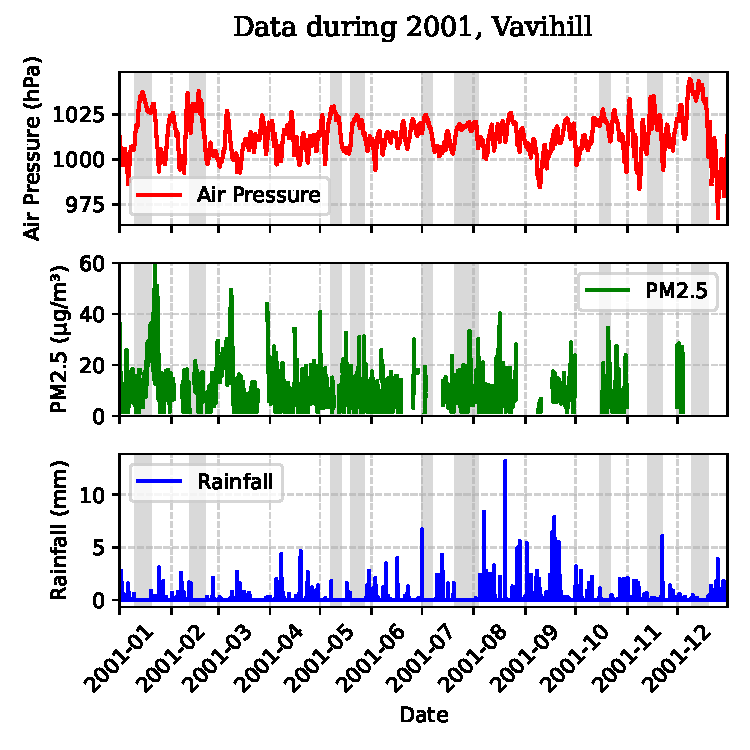
\includegraphics[width=\textwidth]{Figures/Vavihill_plot_20010101_20011231.pdf}
        \label{fig:2001Vavihill}
    \end{subfigure}
    \hfill
    \begin{subfigure}[b]{0.49\textwidth}
        \centering
        \includegraphics[width=\textwidth]{Figures/Malmö_plot_20010101_20011231.pdf}
        \label{fig:2001Malmö}
    \end{subfigure}
    \caption{These example plot displays the air pressure, PM\textsubscript{2.5} concentrations, and rainfall during the year 2001. The periods which was indicated as periods of high-pressure blocking events are shown in gray. }
    \label{fig:2001}
\end{figure}

The second task was to evaluate the PM\textsubscript{2.5} concentrations during periods of high-pressure blocking by taking the mean concentration from the start of the event. This can be seen in \autoref{fig:Meanplot_Comparison}. The data is compared with the PM\textsubscript{2.5} mean taken from periods without high-pressure blocking events. An increase in PM\textsubscript{2.5} concentrations can be seen in Malmö, while a slight increase can be observed in Vavihill. It is important to note that after the first five days, the number of datasets decreases, which is reflected in the increase in standard deviation.


\begin{figure}[H]
    \centering
    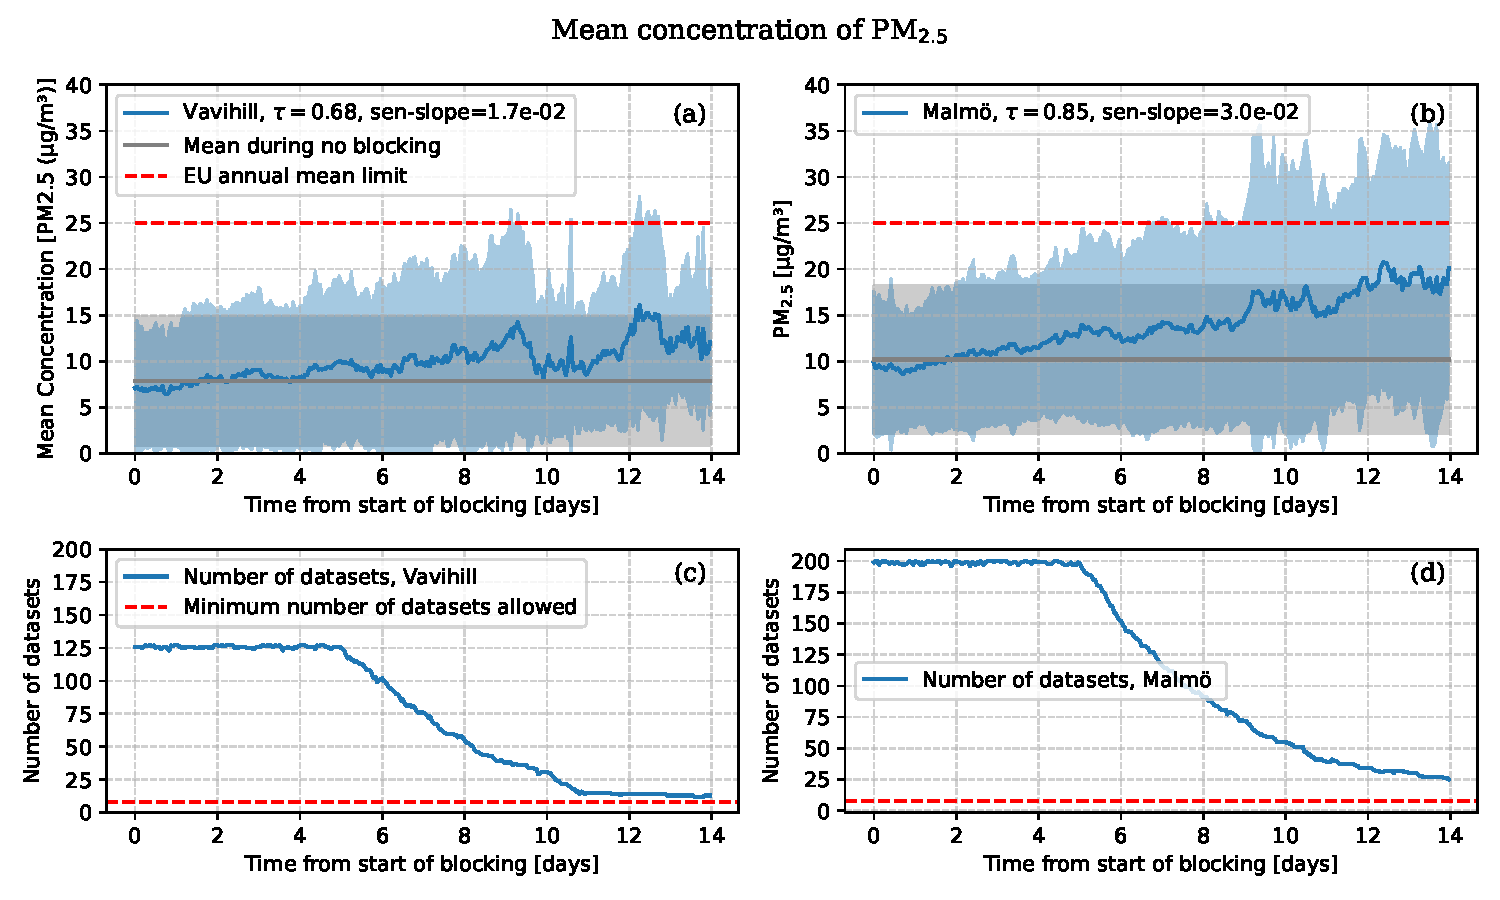
\includegraphics[width=\textwidth]{Figures/Meanplot.pdf}
    \caption{Comparison of mean PM\textsubscript{2.5} concentrations in Vavihill and Malmö, highlighting differences between rural and urban air quality. The shaded region indicates the standard deviation of the data.}
    \label{fig:Meanplot_Comparison}
\end{figure}

The change in PM\textsubscript{2.5} concentrations in Vavihill and Malmö for different wind directions can be seen in \autoref{fig:Meanplot_wind}. One can see similarities between the wind directions for Vavihill and Malmö, although the extremes are more pronounced in Malmö. When the wind filter was applied for the NE direction (310° to 70°), no clear increase or high levels of PM\textsubscript{2.5} were detected. The same is true for the non-specific wind direction in Vavihill. For the other directions, an increase in PM\textsubscript{2.5} can be seen. Elevated levels can also be seen in Vavihill for the SE direction (70° to 190°), in Malmö for the W direction (190° to 310°), and especially in Vavihill for the SE direction (70° to 190°).


\begin{figure}[H]
    \centering
    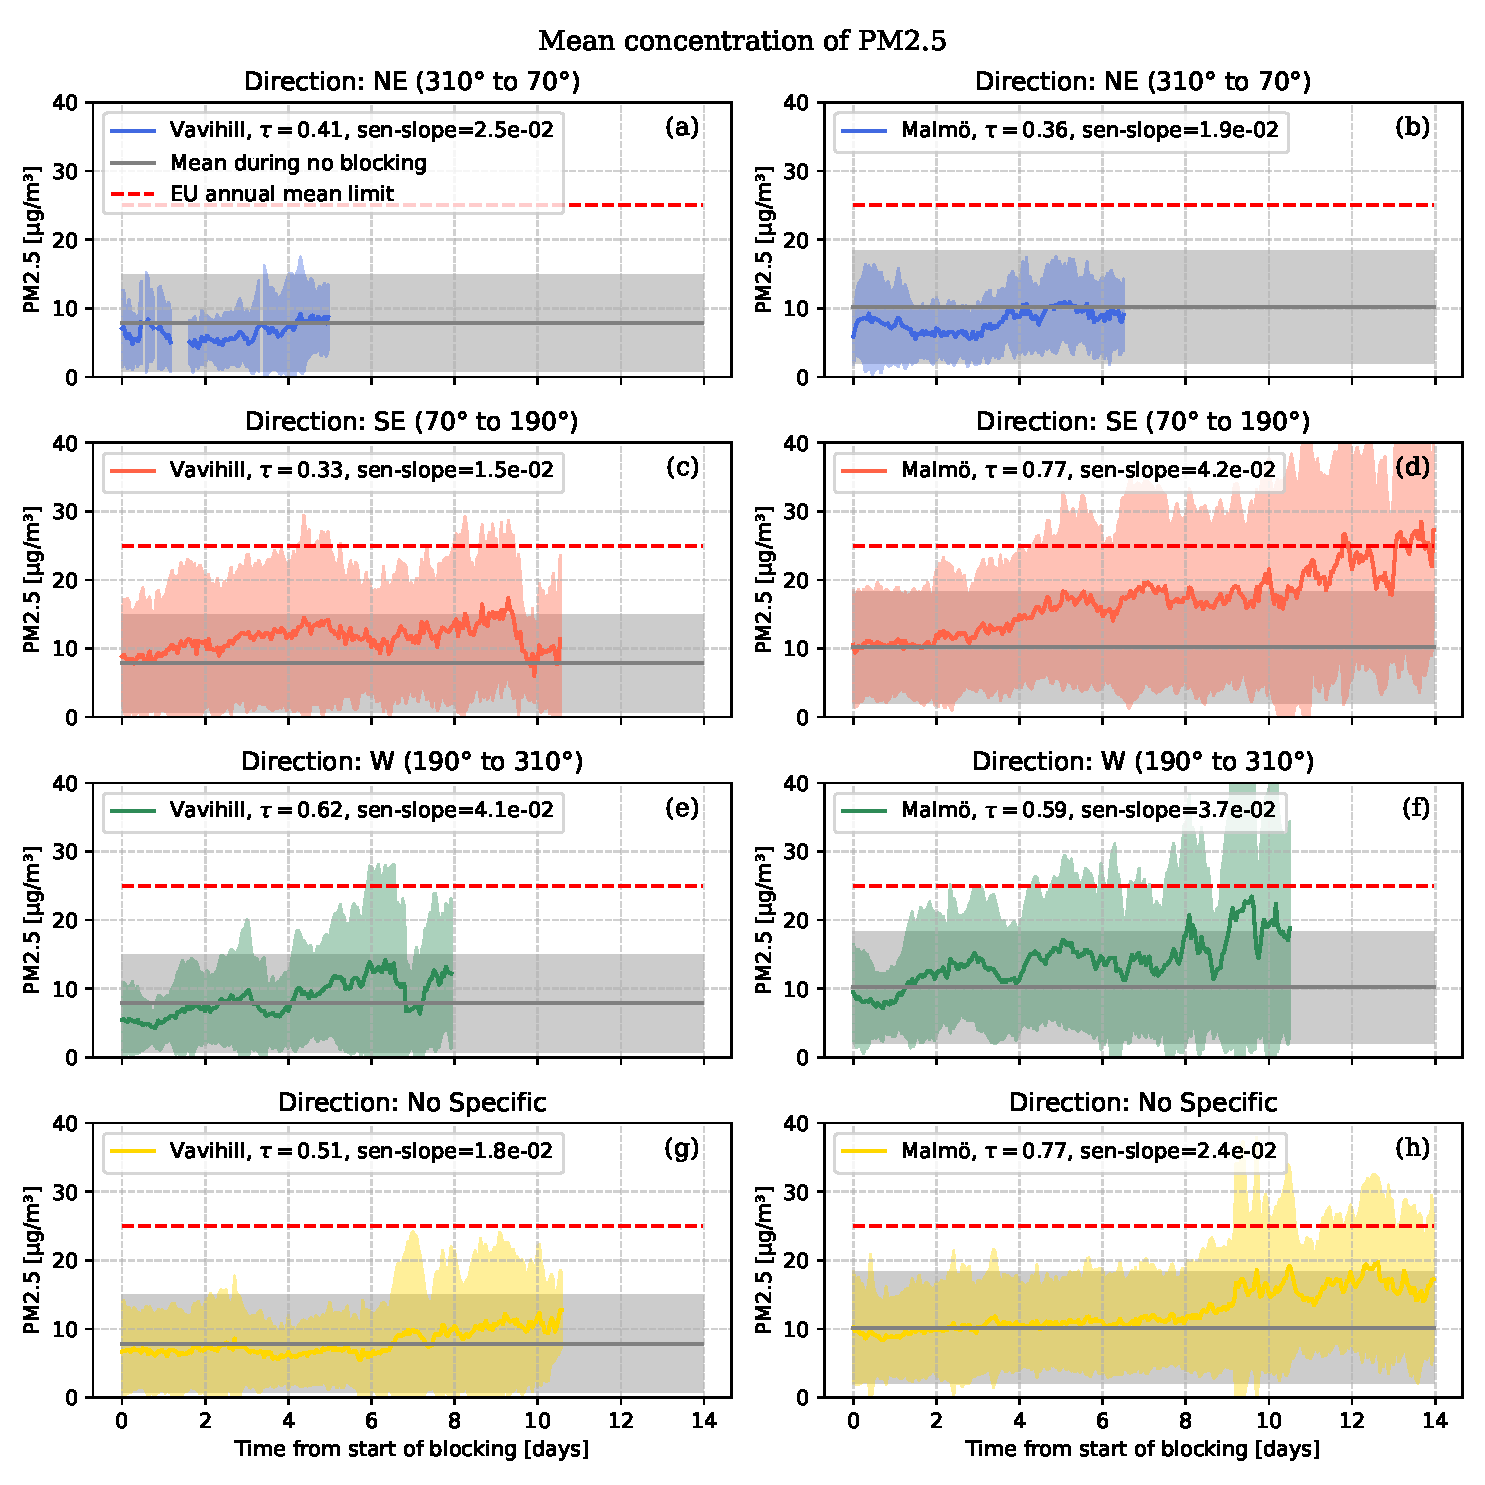
\includegraphics[width=\textwidth]{Figures/Meanplot_dir.pdf}
    \caption{These plots show how PM\textsubscript{2.5} concentrations change in Vavihill and Malmö for different wind directions. In the case of Vavihill, it is important to note that 6.3\% of the winds came from the Northeast (310° to 70°), 39.9\% from the Southeast (70° to 190°), 21.3\% from the West (190° to 310°) and 42.5\% from no specific direction. In the case of Malmö, tt is important to note that 7.5\% of the winds came from the Northeast (310° to 70°), 24.0\% from the Southeast (70° to 190°), 18.5\% from the West (190° to 310°) and 50.0\% from no specific direction. Note that a minimum number of datasets was still put to 8, resulting in some directions having very little data.}
    \label{fig:Meanplot_wind}
\end{figure}


How the concentrations of PM\textsubscript{2.5} changed due to seasonal variation can be seen in \autoref{fig:Meanplot_seasonal}. From these plots, it is clear that the concentration during the summer for both Vavihill and Malmö does not indicate an increase nor high levels of PM\textsubscript{2.5}. A slight increase can be seen in the case of spring for both locations. A larger increase can be seen during the autumn, where high levels of PM\textsubscript{2.5} can be observed towards the end of the period. The winter in Vavihill indicates an increase in the PM\textsubscript{2.5} concentrations, although the standard deviation indicates highly dispersed data. Winter in Malmö indicates an increase in PM\textsubscript{2.5} concentrations, although the levels seem to lower towards the end of the period.

\begin{figure}[H]
    \centering
    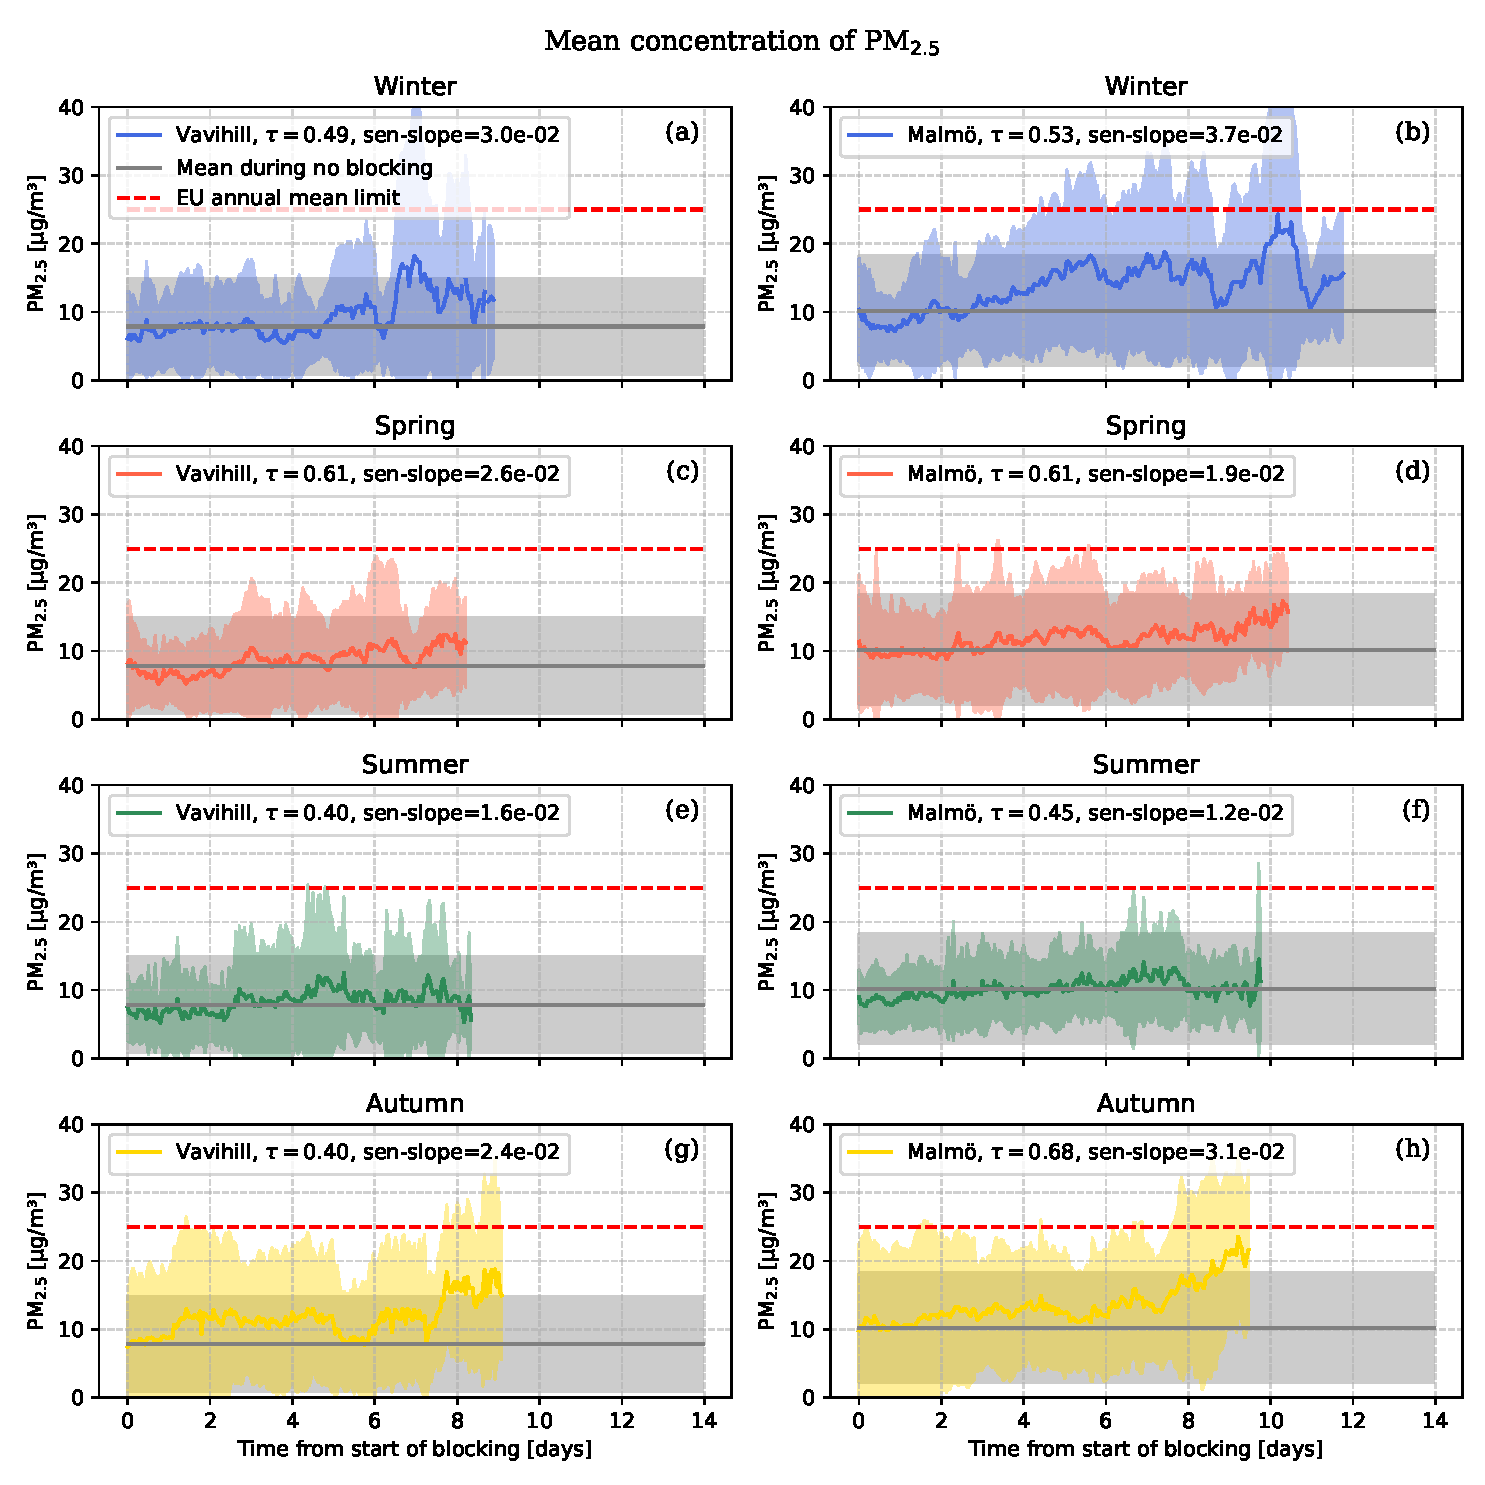
\includegraphics[width=\textwidth]{Figures/Meanplot_seasonal.pdf}
    \caption{These plots show how PM\textsubscript{2.5} concentrations change in Vavihill and Malmö for different seasons. It is important to note that 21.1\% of the blocking events occurred during the winter, 27.4\% during the spring, 24.2\% during the summer and 27.4\% during the autumn. In the case of Malmö, It is important to note that 24.0\% of the blocking events occurred during the winter, 34.0\% during the spring, 18.0\% during the summer and 24.0\% during the autumn. Note that a minimum number of datasets was still put to 8, resulting in some directions having very little data.}
    \label{fig:Meanplot_seasonal}
\end{figure}

The increase in PM\textsubscript{2.5} concentrations depending on the strength of the high-pressure blocking event can be seen in \autoref{fig:Meanplot_pressure}. From the plots, we can observe similar behaviour in the two locations. For weaker and medium-strength high-pressure blocking events, a slight increase in PM\textsubscript{2.5} can be seen, although no significantly elevated concentrations are observed. However, in the case of stronger high-pressure blocking events, a more pronounced increase in PM\textsubscript{2.5} concentrations can be noticed, along with elevated levels of PM\textsubscript{2.5}, especially in Malmö.


\begin{figure}[H]
    \centering
    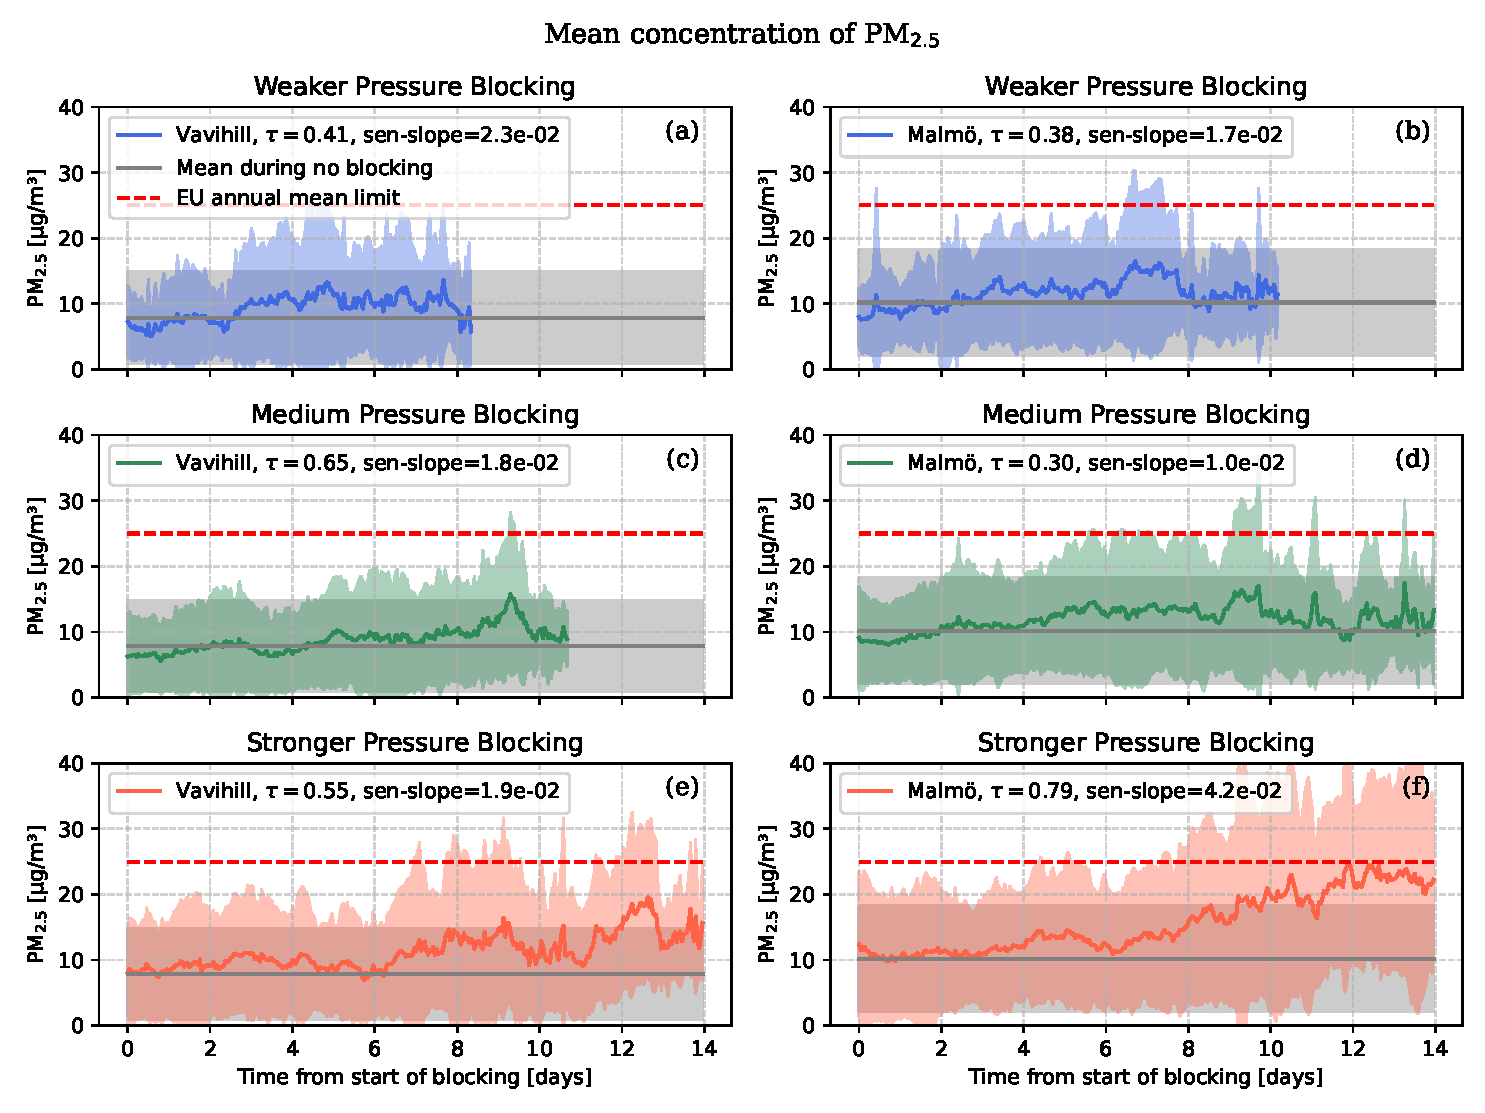
\includegraphics[width=\textwidth]{Figures/Meanplot_pressure.pdf}
    \caption{These plots show how PM\textsubscript{2.5} concentrations change in Vavihill and Malmö for different pressure strengths for high-pressure blocking events. In the case of Vavihill, It is important to note that 20.5\% of the blocking events occurred with a mean pressure below 1020 hPa 44.9\% occurred between 1020 and 1025 hPa and 34.6\% occurred with a mean pressure over 1025hPa. In the cas of Malmö, it is important to note that 17.0\% of the blocking events occurred with a mean pressure below 1020 hPa 48.5\% occurred between 1020 and 1025 hPa and 34.5\% occurred with a mean pressure over 1025hPa. Note that a minimum number of datasets was even here put to 8, resulting in some directions having very little data.}
    \label{fig:Meanplot_pressure}
\end{figure}

The result from the Mann-Kendall test can be viewed in the figures above. All of the categories had a p-value approximately equal to 0. The $\tau$-value can also be viewed. From this, it is clear that the total mean, the western direction, the spring season, and the pressure strengths medium and strong showed a moderate increase in Vavihill. In the case of Malmö, a moderate increase could be seen during the winter season, as well as in the spring, autumn, and stronger pressure events. Even stronger increases could be seen in the total mean, southeastern direction, and the unspecified direction.



\subsection{The frequency of high pressure blocking events}
The last task was to determine whether high-pressure blocking events have become more common. Here the 24 hour rain-limit was set to \SI{4}{\mm}, since this corresponds to little rainfall. When looking at the number of high-pressure blocking events per year, no significant change in frequency could be seen (see \autoref{fig:number_of_blockings}). Since the highest levels of PM\textsubscript{2.5} occurred toward the end of the events (see \autoref{fig:Meanplot_Comparison}, \autoref{fig:Meanplot_wind}, \autoref{fig:Meanplot_seasonal}, and \autoref{fig:Meanplot_pressure}), the frequency of longer high-pressure blocking events was also examined. However, no distinct increase could be observed in any of the cases.

\begin{figure}[H]
    \centering
    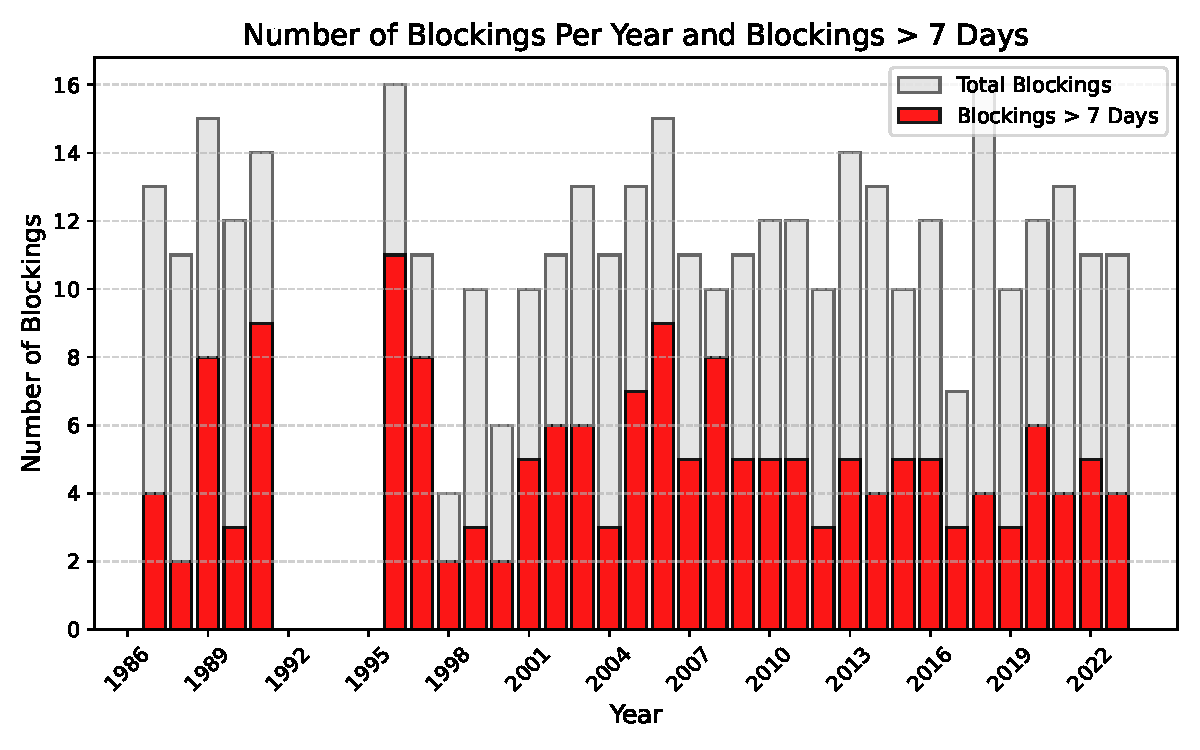
\includegraphics[width=0.7\textwidth]{Figures/BlockingsPerYear.pdf}
    \caption{fig: This plots shows the change in frequency of high-pressure blocking events. The plots also indicates the change in events longer than 7 and 10 days. }
    \label{fig:number_of_blockings}
\end{figure}

In \autoref{fig:Number_of_Blocking_Days_Per_Year}, the number of days under high-pressure blocking events per year can be seen. Here, the total, seasonal, and pressure strength dependence can be observed. The reason for not including the directional dependence is that this was not available from the data. However, these plots show no clear increase or decrease in the number of days under high-pressure blocking events.


\begin{figure}[H]
    \centering
    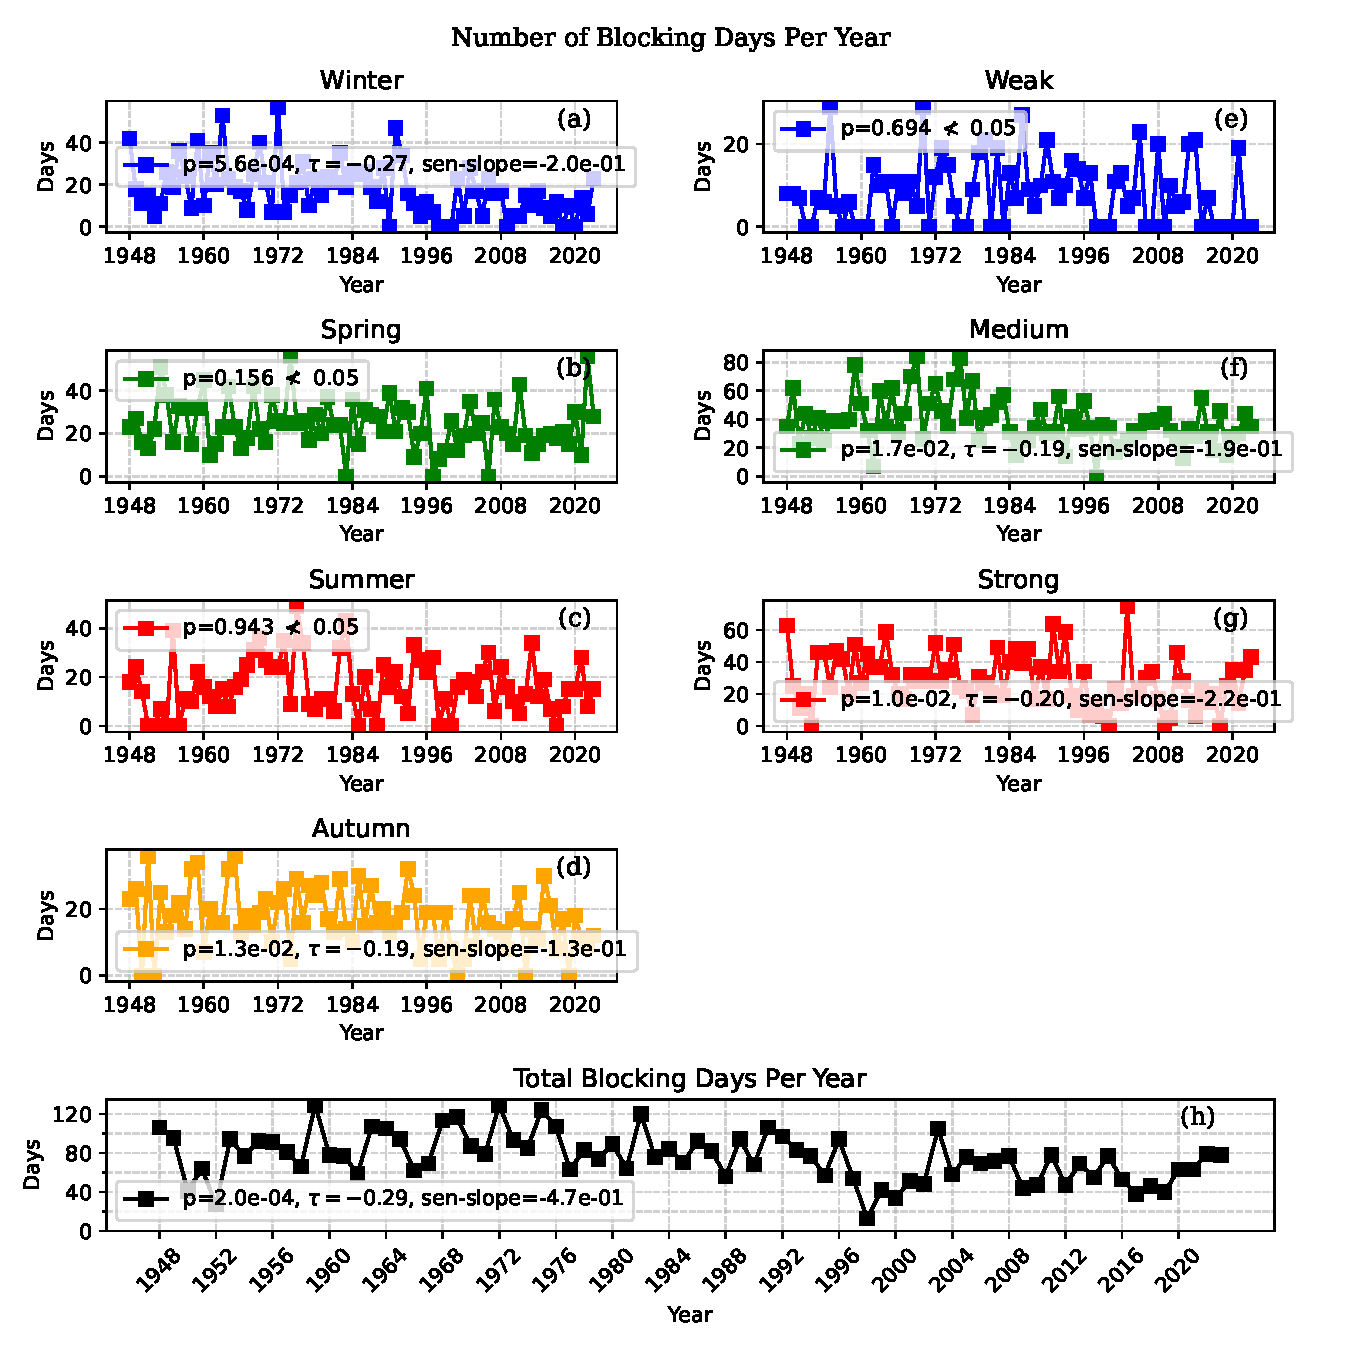
\includegraphics[width=0.8\textwidth]{Figures/blocking_days_per_year_all.pdf}
    \caption{These plots show the change in frequency of days under high-pressure blocking events. The number of days under a high-pressure blocking event each year, during each season, and for different pressure strengths can also be seen.}
    \label{fig:Number_of_Blocking_Days_Per_Year}
\end{figure}






